\chapter{通信中继的数学模型}
\label{cha:com_model}
由于地面终端只能与无人机通信,故在等效图模型中其度为1,先假设地面终端静止,如果存在一种无人机的部署方案使得整部图连通,那么
根据最小生成树的理论,通过去掉一些边仍能保证整部图连通,所以我们只需考虑构造一个树结构使得所有地面终端作为树的叶节点。

采用归纳的方法构造树,先假设对给定的$n$个地面终端已经存在$m$架无人机满足条件。考虑新增一个地面终端$t_j$,
那么我们先考虑离新增的地面终端最近的无人机$a_i$,在不破坏原有树的连通性的前提下移动$a_i$更靠近$t_j$,
如果$a_i$的移动可以满足在与$t_j$通信的范围内,则本轮结束;如果移动完$a_i$仍不能满足要求,顺次考虑其他所有无人机;
如果所有无人机都不能满足要求,保留移动后离$t_j$最近的那架无人机$a_k$的移动方案
并在$a_k$与$t_j$的连线上增加相应数量的
无人机使得条件成立。如此继续下去,可给出全部$N$个地面终端所需的无人机的静态部署方案。

这里问题的难点在于如何刻画“不破坏原有树的连通性”,特别是求出$a_i$可移动的范围。分两种情况考虑:
如果存在某个地面终端通信半径内只有$a_i$,那么$a_i$不能脱离该通信半径$r_{at}$划定的圆;否则则不受此约束。
对于$a_i$所连的任意两架无人机之间的距离如果超过$r_{aa}$,那么该无人机不能脱离两架无人机最大通信圆的相交区域。
可以通过不等式描述这些区域,因此子问题变成如下的平面上的几何优化问题:
\begin{proposition}
设目标点$\bm{P}=(x_0,y_0)$,某地面终端坐标为$(x_1,y_1)$,某其他两架无人机坐标为$(x_2,y_2),(x_3,y_3)$
求解
\begin{equation}\label{bilevel}
\left\{\begin{array}{l}
\min\limits_{{\mbox{\footnotesize\boldmath $x$}}} \sqrt{(x-x_0)^2+(y-y_0)^2}\\[0.2cm]
\mbox{subject to:}\\[0.1cm]
\qquad \left\{\begin{array}{l}
        \sqrt{(x-x_1)^2+(y-y_1)^2}\le r_{at}\\[0.1cm]
        \dots \\[0.1cm]
      \end{array}\right.
\qquad \left\{
    \begin{array}{l}
    \sqrt{(x-x_2)^2+(y-y_2)^2}\le r_{aa}\\[0.2cm]    
    \sqrt{(x-x_3)^2+(y-y_3)^2}\le r_{aa}\\[0.2cm]
    \dots
    \end{array}\right.
\end{array}\right.
\end{equation}
\end{proposition}

实际计算中,由于该子优化问题需要在循环内部调用,实现起来比较复杂,由于时间所限,我们没有完全实现上面描述的算法,而采用的是
当新增加的地面终端的位置不在现有的无人机覆盖范围之内时,在离该地面终端最近的无人机与该地面终端之间增加相应数量的无人机以满足
通信要求。当我们的场景变为动态场景时,只需将无人机与地面终端的通信距离$r_{at}$等效为 1km 即可。

根据简化后的方法求出的无人机的部署方案如下图所示:
\begin{figure}[!ht]\label{fig:communicaton}
\centering
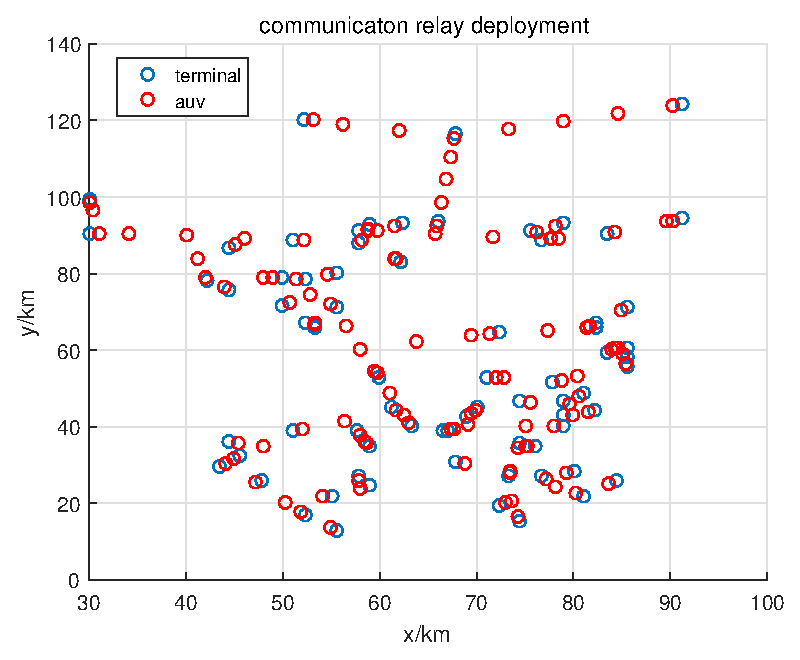
\includegraphics[width=10cm]{communicaton_relay_deployment.eps}
\caption{无人机的部署方案}
\end{figure}

所需的无人机数量是115架,这是一个上界。
